\documentclass[portrait]{seminar}
%\usepackage{pandora}
\usepackage{color}
\usepackage{fancybox}
\usepackage{alltt}
\usepackage{epsfig}
\usepackage{rail}
\usepackage{bar}
\usepackage{url}
\usepackage{rotating}
\usepackage[normalem]{ulem}
\usepackage{latexsym}
\usepackage{amsmath}

\begin{document}

\boldmath
\newcommand{\RA}{$\rightarrow$}
\newcommand{\LL}{\mbox{$[$\hspace{-0.15em}$[$}}
\newcommand{\RR}{\mbox{$]$\hspace{-0.15em}$]$}}
\newcommand{\CC}[1]{\mbox{\tt $\LL$#1$\RR$}}

\slideframe{shadow}

%%% Activate one of these to get either Aarhus style or McGill style 
%%% by putting a #1 in the appropriate line.
\newcommand{\mcgill}[1]{#1}
\newcommand{\aarhus}[1]{}

%%% Define this to be the name of your term
\newcommand{\courseterm}{Fall 2012}




\aarhus{
\newpagestyle{dOvsstyle}{dOvs'98 Week 43 \hfil Type checking}{\hfil \thepage}
}

\mcgill{
\newpagestyle{dOvsstyle}{COMP 520 \courseterm  \hfil Type checking (\thepage)}{}
}
\slidepagestyle{dOvsstyle}

\begin{slide*}
\begin{tabbing}
\aarhus{{\Large\bf Week 43}\\}
~\\
{\Huge\bf Type checking}\\
\end{tabbing}

\vspace{0.4in}

\begin{center}
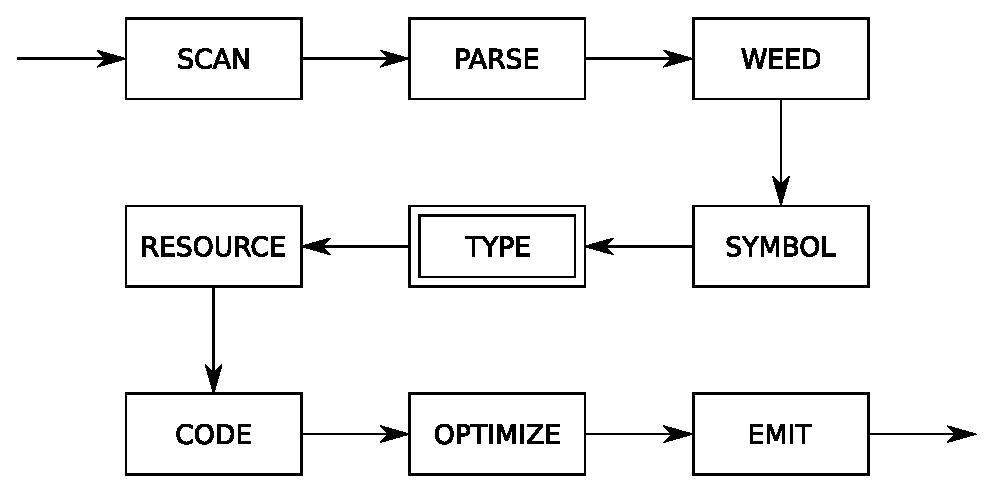
\psfig{file=figs/type.eps,width=20em}
\end{center}

\vfil
\end{slide*}
 
\begin{slide*}
The {\em type checker\/} has severals tasks:
\begin{itemize}
\item determine the types of all expressions;
\item check that values and variables are used correctly; and
\item resolve certain ambiguities by transforming the program.
\end{itemize}

Some languages have no type checker.

\vfil
\end{slide*}
 
\begin{slide*}
A {\em type\/} describes possible values.

The JOOS types are:
\begin{itemize}
\item {\tt void}: the empty type;
\item {\tt int}: the integers;
\item {\tt char}: the characters;
\item {\tt boolean}: {\tt true} and {\tt false}; and
\item {\tt C}: objects of class {\tt C} or any subclass.
\end{itemize}
Plus an artificial type:
\begin{itemize}
\item {\tt polynull}
\end{itemize}
which is the type of the polymorphic {\tt null} constant.

\vfil
\end{slide*}

\begin{slide*}
A {\em type annotation}:

\begin{verbatim} 
int x;
Cons y;
\end{verbatim}

specifies an {\em invariant\/} about the run-time behavior:

\begin{itemize}
\item {\tt x} will always contain an integer value; and
\item {\tt y} will always contain {\tt null} or an object of type {\tt Cons}
or any subclass.
\end{itemize}

Usual type annotations are not very expressive as invariants.

You can have types without annotations, through type inference (e.g. in ML).

Types can be arbitrarily complex in theory.
\vfil
\end{slide*}
 
\begin{slide*}
A program is {\em type correct\/} if the type annotations are
valid invariants.

Type correctness is undecidable:

\begin{alltt}
int x;
int j;

x = 0;
scanf("%i",&j);
TM(j);
x = true;
\end{alltt}

where {\tt TM(j)} simulates the {\tt j}'th Turing machine on empty input.

The program is type correct if and only if {\tt TM(j)} does not halt on empty input.
\vfil
\end{slide*}
 
\begin{slide*}
A program is {\em statically\/} type correct if it satisfies some type rules.

The type rules are chosen to be:
\begin{itemize}
\item simple to understand;
\item efficient to decide; and
\item conservative with respect to type correctness.
\end{itemize}

Type rules are rarely canonical.
\vfil
\end{slide*}
 
\begin{slide*}
Static type systems are necessarily flawed:\\

\setlength{\unitlength}{0.0006200in}%
%
\begingroup\makeatletter\ifx\SetFigFont\undefined%
\gdef\SetFigFont#1#2#3#4#5{%
  \reset@font\fontsize{#1}{#2pt}%
  \fontfamily{#3}\fontseries{#4}\fontshape{#5}%
  \selectfont}%
\fi\endgroup%
\begin{picture}(3758,2124)(1726,-4048)
\thicklines
\put(3901,-2911){\circle{670}}
\put(3676,-3361){\circle*{100}}
\put(3901,-2461){\line(-3, 1){450}}
\put(3451,-2311){\line( 1,-5){ 75}}
\put(3526,-2686){\line(-1, 0){375}}
\put(3151,-2686){\line( 3,-2){225}}
\put(3376,-2836){\line(-4,-3){300}}
\put(3076,-3061){\line( 6,-1){450}}
\put(3526,-3136){\line(-3,-2){225}}
\put(3301,-3286){\line( 3,-2){225}}
\put(3526,-3436){\line(-1,-2){150}}
\put(3376,-3736){\line( 5, 3){375}}
\put(3751,-3511){\line( 2,-1){300}}
\put(4051,-3661){\line( 1, 5){ 75}}
\put(4126,-3286){\line( 5,-3){375}}
\put(4501,-3511){\line(-3, 5){225}}
\put(4276,-3136){\line( 6,-1){450}}
\put(4726,-3211){\line(-5, 4){375}}
\put(4351,-2911){\line( 5, 1){375}}
\put(4726,-2836){\line(-6, 1){450}}
\put(4276,-2761){\line( 1, 1){300}}
\put(4576,-2461){\line(-5,-2){375}}
\put(4201,-2611){\line(-1, 6){ 75}}
\put(4126,-2161){\line(-3,-4){225}}
\put(2251,-2686){\vector( 4,-1){1200}}
\put(2851,-4036){\framebox(2100,2100){}}
\put(5472,-2593){\vector(-4,-1){1500}}
\put(1726,-2611){\makebox(0,0)[lb]{\smash{\SetFigFont{6}{14.4}{\familydefault}{\mddefault}{\updefault}type correct}}}
\put(5101,-2536){\makebox(0,0)[lb]{\smash{\SetFigFont{6}{14.4}{\familydefault}{\mddefault}{\updefault}statically type correct}}}
\end{picture}

There is always {\em slack}, i.e. programs that are unfairly
rejected by the type checker.  Some are even quite useful.

Can you think of such a program?

%% \begin{verbatim}
 
%% int x;

%% x = 87;
%% if (false) x = true;

%% \end{verbatim}

\vfil
\end{slide*}
 
\begin{slide*}
Type rules may be specified:

\begin{itemize}
\item in ordinary prose:\\
\begin{small}
{\tt The argument to the sqrt function must be of type int; the result is of type real.}
\end{small}
\item as constraints on type variables:
\begin{center}
{\tt sqrt(x): \LL{}sqrt(x)\RR{}$=$real $\wedge$ \LL{}x\RR{}$=$int}
\end{center}
\item as logical rules:
$$ \frac{{\cal S} \vdash \mbox{\tt x}: \mbox{\tt int}}{{\cal S} \vdash \mbox{\tt sqrt(x)}: \mbox{\tt real}}$$
\end{itemize}

There are always three kinds:
\begin{enumerate}
\item declarations: introduction of variables;
\item propagations: expression type determines enclosing expression
type; and
\item restrictions: expression type constrained by usage context
\end{enumerate}
\vfil
\end{slide*}

\newcommand{\lib}{\mbox{$L$}}
\newcommand{\class}{\mbox{$C$}}
\newcommand{\method}{\mbox{$M$}}
\newcommand{\vars}{\mbox{$V$}}
 
\begin{slide*}
The judgement for statements:
$$ \lib{},\class{},\method{},\vars{} \vdash S $$

means that $S$ is statically type correct with:

\begin{itemize}
\item class library \lib{};
\item current class \class{};
\item current method \method{}; and
\item variables \vars{}.
\end{itemize}

The judgement for expressions:
$$ \lib{},\class{},\method{},\vars{} \vdash E: \tau $$
 
means that $E$ is statically type correct and has type $\tau$.

The tuple $\lib{},\class{},\method{},\vars{}$ is an abstraction of the symbol table.
\vfil
\end{slide*}
 
\begin{slide*}
Type rules for statement sequence:

$$ \frac{\lib{},\class{},\method{},\vars{} \vdash S_1\;\;\;\;\;
         \lib{},\class{},\method{},\vars{} \vdash S_2}{
        \lib{},\class{},\method{},\vars{} \vdash S_1\; S_2} $$
$$ \frac{\lib{},\class{},\method{},\vars{}[\mbox{\tt x} \mapsto \tau] \vdash S}{
         \lib{},\class{},\method{},\vars{} \vdash \tau\;\; \mbox{\tt x;} S}$$

$\vars{}[\mbox{\tt x} \mapsto \tau]$ just says ${\tt x}$ maps to
        $\tau$ within $\vars{}$.

Corresponding JOOS source:

\begin{scriptsize}
\begin{verbatim}

case sequenceK:
     typeImplementationSTATEMENT(s->val.sequenceS.first,
                                 class,returntype);
     typeImplementationSTATEMENT(s->val.sequenceS.second,
                                 class,returntype);
     break;
.
.
.

case localK:
     break;
\end{verbatim}
\end{scriptsize}
\vfil
\end{slide*}
 
\begin{slide*}
Type rules for return statements:

$$ \frac{\mbox{\em type}(\lib{},\class{},\method{}) = \mbox{\tt void}}{
         \lib{},\class{},\method{},\vars{} \vdash \mbox{\tt return}} $$
$$ \frac{\lib{},\!\class{},\!\method{},\!\vars{} \vdash E\!: \tau\;\;
         \mbox{\em type}(\lib{},\!\class{},\!\method{})\!=\!\sigma\;\; \sigma\!:=\!\tau}{
         \lib{},\class{},\method{},\vars{} \vdash \mbox{\tt return}\; E} $$

$\sigma\!:=\!\tau$ just says something of type $\sigma$ can be
assigned something of type $\tau$.

Corresponding JOOS source:
 
\begin{scriptsize}
\begin{verbatim}

case returnK:
  if (s->val.returnS!=NULL) {
     typeImplementationEXP(s->val.returnS,class);
  }
  if (returntype->kind==voidK && s->val.returnS!=NULL) {
     reportError("return value not allowed",s->lineno);
  }
  if (returntype->kind!=voidK && s->val.returnS==NULL) {
     reportError("return value expected",s->lineno);
  }
  if (returntype->kind!=voidK && s->val.returnS!=NULL) {
     if (!assignTYPE(returntype,s->val.returnS->type)) {
        reportError("illegal type of expression",
                    s->lineno);
     }
  }
  break;
\end{verbatim}
\end{scriptsize}

\vfil
\end{slide*}
 
\begin{slide*}
Assignment compatibility:

\begin{itemize}
\item {\tt int$:=$int};
\item {\tt int$:=$char};
\item {\tt char$:=$char};
\item {\tt boolean$:=$boolean};
\item {\tt C$:=$polynull}; and
\item {\tt C$:=$D}, if {\tt D} $\leq$ {\tt C}.
\end{itemize}

\begin{center}
\setlength{\unitlength}{0.00041500in}%
%
\begingroup\makeatletter\ifx\SetFigFont\undefined%
\gdef\SetFigFont#1#2#3#4#5{%
  \reset@font\fontsize{#1}{#2pt}%
  \fontfamily{#3}\fontseries{#4}\fontshape{#5}%
  \selectfont}%
\fi\endgroup%
\begin{picture}(3324,2658)(2239,-4648)
\thicklines
\put(3901,-2161){\line(-2,-3){1650}}
\put(3901,-2161){\line( 2,-3){1650}}
\put(3901,-2161){\line(-2,-5){300}}
\put(3601,-2911){\line( 2,-1){450}}
\put(4051,-3136){\line(-4,-3){600}}
\put(3451,-3586){\line( 4,-1){600}}
\put(3826,-2086){\makebox(0,0)[lb]{\smash{\SetFigFont{8}{14.4}{\ttdefault}{\mddefault}{\updefault}C}}}
\put(4051,-3886){\makebox(0,0)[lb]{\smash{\SetFigFont{8}{14.4}{\ttdefault}{\mddefault}{\updefault}D}}}
\end{picture}
\end{center}

Corresponding JOOS source:
 
\begin{scriptsize}
\begin{verbatim}
int assignTYPE(TYPE *s, TYPE *t)
{ if (s->kind==refK && t->kind==polynullK) return 1;
  if (s->kind==intK && t->kind==charK) return 1;
  if (s->kind!=t->kind) return 0;
  if (s->kind==refK) return subClass(t->class,s->class);
  return 1;
}
\end{verbatim}
\end{scriptsize}

\vfil
\end{slide*}
 
\begin{slide*}
Type rule for expression statements:

$$ \frac{\lib{},\class{},\method{},\vars{} \vdash E: \tau}{
        \lib{},\class{},\method{},\vars{} \vdash E} $$

Corresponding JOOS source:
 
\begin{scriptsize}
\begin{verbatim}

case expK:
     typeImplementationEXP(s->val.expS,class);
     break;

\end{verbatim}
\end{scriptsize}

Type rule for {\tt if}-statement:
$$ \frac{\lib{},\class{},\method{},\vars{} \vdash E: \mbox{\tt boolean}\;\;\;\;
         \lib{},\class{},\method{},\vars{} \vdash S}{
         \lib{},\class{},\method{},\vars{} \vdash \mbox{\tt if (}E\mbox{\tt )}\;S} $$

Corresponding JOOS source:
 
\begin{scriptsize}
\begin{verbatim}
 
case ifK:
   typeImplementationEXP(s->val.ifS.condition,class);
   checkBOOL(s->val.ifS.condition->type,s->lineno);
   typeImplementationSTATEMENT(s->val.ifS.body,
                               class,returntype);
   break;

\end{verbatim}
\end{scriptsize}
\vfill
\end{slide*}
 
\begin{slide*}
Type rule for variables:

$$ \frac{\vars{}(\mbox{\tt x}) = \tau}{
         \lib{},\class{},\method{},\vars{} \vdash \mbox{\tt x}: \tau} $$

Corresponding JOOS source:
 
\begin{scriptsize}
\begin{verbatim}
 
case idK:
     e->type = typeVar(e->val.idE.idsym);
     break;

\end{verbatim}
\end{scriptsize}
 
Type rule for assignment:

$$ \frac{\lib{},\!\class{},\!\method{},\!\vars{} \vdash \mbox{\tt x}\!:\tau\;\;
         \lib{},\!\class{},\!\method{},\!\vars{} \vdash E\!:\sigma\;\; \tau:=\sigma}{
         \lib{},\!\class{},\!\method{},\!\vars{} \vdash \mbox{\tt x=}E: \tau} $$

Corresponding JOOS source:
 
\begin{scriptsize}
\begin{verbatim}
 
case assignK:
   e->type = typeVar(e->val.assignE.leftsym);
   typeImplementationEXP(e->val.assignE.right,class);
   if (!assignTYPE(e->type,e->val.assignE.right->type)) {
      reportError("illegal assignment",e->lineno);
   }
   break;
 
\end{verbatim}
\end{scriptsize}

\vfil
\end{slide*}

\begin{slide*} 
Type rule for minus:

$$ \frac{\lib{},\!\class{},\!\method{},\!\vars{} \vdash E_1: \mbox{\tt int}\;\;\;\;
         \lib{},\!\class{},\!\method{},\!\vars{} \vdash E_2: \mbox{\tt int}}{
         \lib{},\!\class{},\!\method{},\!\vars{} \vdash E_1 \mbox{\tt -} E_2: \mbox{\tt int}} $$

Corresponding JOOS source:
 
\begin{scriptsize}
\begin{verbatim}
case minusK:
     typeImplementationEXP(e->val.minusE.left,class);
     typeImplementationEXP(e->val.minusE.right,class);
     checkINT(e->val.minusE.left->type,e->lineno);
     checkINT(e->val.minusE.right->type,e->lineno);
     e->type = intTYPE;
     break;
\end{verbatim}
\end{scriptsize}

Implicit integer cast:

$$ \frac{\lib{},\!\class{},\!\method{},\!\vars{} \vdash E: \mbox{\tt char}}{
         \lib{},\!\class{},\!\method{},\!\vars{} \vdash E: \mbox{\tt int}} $$

Corresponding JOOS source:

\begin{scriptsize}
\begin{verbatim}
int checkINT(TYPE *t, int lineno)
{ if (t->kind!=intK && t->kind!=charK) {
     reportError("int type expected",lineno);
     return 0;
  }
  return 1;
}
\end{verbatim}
\end{scriptsize}

\vfil
\end{slide*}
 
\begin{slide*}
Type rule for equality:

%\vspace{1.5in}

$$ \frac{\begin{array}{l}
          \lib{},\!\class{},\!\method{},\!\vars{} \vdash E_1: \tau_1\\
          \lib{},\!\class{},\!\method{},\!\vars{} \vdash E_2: \tau_2\\
          \tau_1:=\tau_2\,\vee\,\tau_2:=\tau_1\end{array}}{
          \lib{},\!\class{},\!\method{},\!\vars{} \vdash E_1 \mbox{\tt ==} E_2: \mbox{\tt boolean}} $$\\

Corresponding JOOS source:
 
\begin{scriptsize}
\begin{verbatim}
 
case eqK:
     typeImplementationEXP(e->val.eqE.left,class);
     typeImplementationEXP(e->val.eqE.right,class);
     if (!assignTYPE(e->val.eqE.left->type,
                     e->val.eqE.right->type) &&
         !assignTYPE(e->val.eqE.right->type,
                     e->val.eqE.left->type)) {
        reportError("arguments for == have wrong types",
                    e->lineno);
     }
     e->type = boolTYPE;
     break;
 
\end{verbatim}
\end{scriptsize}
        
\vfil
\end{slide*}
 
\begin{slide*}
Type rule for {\tt this}:

$$ \lib{},\!\class{},\!\method{},\!\vars{} \vdash \mbox{\tt this}: \class{} $$

Corresponding JOOS source:
 
\begin{scriptsize}
\begin{verbatim}
 
case thisK:
     if (class==NULL) {
        reportError("'this' not allowed here",e->lineno);
     }
     e->type = classTYPE(class);
     break;
 
\end{verbatim}
\end{scriptsize}
 
\vfil
\end{slide*}
 
\begin{slide*}

Type rule for cast:

$$ \frac{\lib{},\!\class{},\!\method{},\!\vars{} \vdash E: \tau\;\;\;\;
         \tau\leq\mbox{\tt C}\, \vee \,\mbox{\tt C}\leq\tau
        }{
         \lib{},\!\class{},\!\method{},\!\vars{} \vdash \mbox{\tt (C)}E:\; \mbox{\tt C}
        } $$

Corresponding JOOS source:
 
\begin{scriptsize}
\begin{verbatim}
 
case castK:
     typeImplementationEXP(e->val.castE.right,class);
     e->type = makeTYPEextref(e->val.castE.left,
                              e->val.castE.class);
     if (e->val.castE.right->type->kind!=refK &&
         e->val.castE.right->type->kind!=polynullK) {
        reportError("class reference expected",e->lineno);
     } else {
        if (e->val.castE.right->type->kind==refK &&
            !subClass(e->val.castE.class,
                      e->val.castE.right->type->class) &&
            !subClass(e->val.castE.right->type->class,
                      e->val.castE.class)) {
           reportError("cast will always fail",e->lineno);
        }
     }
     break;

\end{verbatim}
\end{scriptsize}


\vfil
\end{slide*}
 
\begin{slide*}
 
Type rule for {\tt instanceof}:

$$ \frac{\lib{},\!\class{},\!\method{},\!\vars{} \vdash E: \tau\;\;\;\;
         \tau\leq \mbox{\tt C}\, \vee \,\mbox{\tt C}\leq \tau}{
        \lib{},\!\class{},\!\method{},\!\vars{} \vdash E\; \mbox{\tt instanceof C}: \mbox{\tt
boolean}} $$

Corresponding JOOS source:
 
\begin{scriptsize}
\begin{verbatim}
 
case instanceofK:
   typeImplementationEXP(e->val.instanceofE.left,class);
   if (e->val.instanceofE.left->type->kind!=refK) {
      reportError("class reference expected",e->lineno);
   } 
   if (!subClass(e->val.instanceofE.left->type->class,
                 e->val.instanceofE.class) &&
       !subClass(e->val.instanceofE.class,
                 e->val.instanceofE.left->type->class)) {
      reportError("instanceof will always fail",e->lineno);
   }
   e->type = boolTYPE;
   break;

\end{verbatim}
\end{scriptsize}

\vfil
\end{slide*}

\begin{slide*}
Why the predicate:

$$ \tau\leq \mbox{\tt C}\, \vee \,\mbox{\tt C}\leq \tau $$

for ``$\mbox{\tt (C)}E$'' and ``$E\; \mbox{\tt instanceof C}$''?\\

\renewcommand{\arraystretch}{1.5}
\begin{tabular}{lll}
\setlength{\unitlength}{0.0004in}%
%
\begingroup\makeatletter\ifx\SetFigFont\undefined%
\gdef\SetFigFont#1#2#3#4#5{%
  \reset@font\fontsize{#1}{#2pt}%
  \fontfamily{#3}\fontseries{#4}\fontshape{#5}%
  \selectfont}%
\fi\endgroup%
\begin{picture}(1516,912)(1643,-2017)
\thicklines
\put(2401,-1561){\oval(1500,900)}
\put(2101,-1561){\circle{540}}
\put(2000,-1656){\makebox(0,0)[lb]{\smash{\SetFigFont{12}{14.4}{\ttdefault}{\mddefault}{\updefault}$\tau$}}}
\put(2626,-1656){\makebox(0,0)[lb]{\smash{\SetFigFont{12}{14.4}{\ttdefault}{\mddefault}{\updefault}C}}}
\end{picture}
  & \raisebox{2ex}{succeeds} & \raisebox{2ex}{$\tau\leq \mbox{\tt C}$} \\


\setlength{\unitlength}{0.0004in}%
%
\begingroup\makeatletter\ifx\SetFigFont\undefined%
\gdef\SetFigFont#1#2#3#4#5{%
  \reset@font\fontsize{#1}{#2pt}%
  \fontfamily{#3}\fontseries{#4}\fontshape{#5}%
  \selectfont}%
\fi\endgroup%
\begin{picture}(1651,1124)(1013,-2198)
\thicklines
\put(1501,-1561){\circle{960}}
\put(2176,-1711){\circle{960}}
\put(2176,-1799){\makebox(0,0)[lb]{\smash{\SetFigFont{12}{14.4}{\rmdefault}{\mddefault}{\updefault}{\tt C}}}}
\put(1326,-1636){\makebox(0,0)[lb]{\smash{\SetFigFont{12}{14.4}{\rmdefault}{\mddefault}{\updefault}$\tau$}}}
\end{picture}
  &  \raisebox{2ex}{really useful} &  \raisebox{2ex}{$\mbox{\tt C}\leq \tau$}\\

\setlength{\unitlength}{0.0004in}%
%
\begingroup\makeatletter\ifx\SetFigFont\undefined%
\gdef\SetFigFont#1#2#3#4#5{%
  \reset@font\fontsize{#1}{#2pt}%
  \fontfamily{#3}\fontseries{#4}\fontshape{#5}%
  \selectfont}%
\fi\endgroup%
\begin{picture}(2176,974)(1013,-2048)
\thicklines
\put(1501,-1561){\circle{960}}
\put(2701,-1561){\circle{960}}
\put(1400,-1636){\makebox(0,0)[lb]{\smash{\SetFigFont{12}{14.4}{\rmdefault}{\mddefault}{\updefault}$\tau$}}}
\put(2606,-1656){\makebox(0,0)[lb]{\smash{\SetFigFont{12}{14.4}{\rmdefault}{\mddefault}{\updefault}{\tt C}}}}
\end{picture}
  &  \raisebox{2ex}{fails} & \raisebox{2ex}{$\tau\not\leq \mbox{\tt C} \wedge \mbox{\tt C}\not\leq \tau $}
\end{tabular}
\renewcommand{\arraystretch}{1}
\\[2ex]
Circle denotes type and all its subtypes. For instance, the following would
fail to type check, as no subtype of \verb$List$ can ever be a subtype of the
final (!) class \verb$String$:
\begin{verbatim}
List l;
if(l instanceof String) ... 
\end{verbatim}
\vfil
\end{slide*}

\begin{slide*}
Type rule for method invocation:
$$ \frac{\begin{array}{l}
      \lib{},\class{},\method{},\vars{} \vdash E: \sigma \wedge \sigma \in \lib{}\\
      \exists\, \rho\!: \sigma \leq \rho \wedge \mbox{\tt m} \in \mbox{\em
      methods}(\rho)\\
      \neg \mbox{\em static}(\mbox{\tt m})\\
      \lib{},\class{},\method{},\vars{} \vdash E_i: \sigma_i\\
      \mbox{\em argtype}(\lib{},\rho,\mbox{\tt m},i) := \gamma_i \wedge \gamma_i := \sigma_i\\
      \mbox{\em type}(\lib{},\rho{},\mbox{\tt m}) = \tau
   \end{array}}{
       \lib{},\class{},\method{},\vars{} \vdash E\mbox{\tt .m(}E_1,\ldots,E_n\mbox{\tt )}: \tau
   }
$$
 
\vfil
\end{slide*}
 
\begin{slide*}
Corresponding JOOS source:
 
\begin{scriptsize}
\begin{verbatim}
 
case invokeK:
   t = typeImplementationRECEIVER(
           e->val.invokeE.receiver,class);
   typeImplementationARGUMENT(e->val.invokeE.args,class);
   if (t->kind!=refK) {
      reportError("receiver must be an object",e->lineno);
      e->type = polynullTYPE;
   } else {
      s = lookupHierarchy(e->val.invokeE.name,t->class);
      if (s==NULL || s->kind!=methodSym) {
         reportStrError("no such method called %s",
                        e->val.invokeE.name,e->lineno);
         e->type = polynullTYPE;
      } else {
         e->val.invokeE.method = s->val.methodS;
         if (s->val.methodS.modifier==modSTATIC) {
            reportStrError(
                  "static method %s may not be invoked",
                  e->val.invokeE.name,e->lineno);
         }
         typeImplementationFORMALARGUMENT(
             s->val.methodS->formals,
             e->val.invokeE.args,e->lineno);
         e->type = s->val.methodS->returntype;
      }
   }
   break;
\end{verbatim}
\end{scriptsize}
\vfil
\end{slide*}

\begin{slide*}
Type rule for constructor invocation:
\renewcommand{\arraystretch}{0.95}
$$ \frac{\begin{array}{l}
      \lib{},\class{},\method{},\vars{} \vdash E_i: \sigma_i\\[1ex]
      \exists\, \vec{\tau}\!:\!\!\begin{array}[t]{l}\mbox{\em constructor}(\lib{},\mbox{\tt C},\vec{\tau})\; \wedge\\
              \vec{\tau}:=\vec{\sigma}\; \wedge\\
              (\forall \vec{\gamma}\!:\begin{array}[t]{l}\mbox{\em constructor}(\lib{},\mbox{\tt C},\vec{\gamma}) \wedge \vec{\gamma}:=\vec{\sigma}\\
                       \Downarrow \\ \vec{\gamma}:=\vec{\tau}\end{array}\\)\end{array}\\
   \end{array}}{
       \lib{},\class{},\method{},\vars{} \vdash \mbox{\tt new C(}E_1,\ldots,E_n\mbox{\tt )}: \mbox{\tt C}
   }
$$
\renewcommand{\arraystretch}{1}

Corresponding JOOS source:

\begin{scriptsize}
\begin{verbatim}
case newK:
     if (e->val.newE.class->modifier==modABSTRACT) {
         reportStrError("illegal abstract constructor %s",
                         e->val.newE.class->name,
                         e->lineno);
     }
     typeImplementationARGUMENT(e->val.newE.args,this);
     e->val.newE.constructor = 
        selectCONSTRUCTOR(e->val.newE.class->constructors,
                          e->val.newE.args,
                          e->lineno);
     e->type = classTYPE(e->val.newE.class);
     break;

\end{verbatim}
\end{scriptsize}
\vfil
\end{slide*}

\begin{slide*}
Different kinds of type rules are:
\begin{itemize}
\item {\em axioms}:
\end{itemize}
      $$\lib{},\class{},\method{},\vars{} \vdash \mbox{\tt this}: \class{}$$
\begin{itemize}
\item {\em predicates}:
\end{itemize}
      $$\tau\leq\mbox{\tt C} \,\vee\, \mbox{\tt C}\leq\tau$$
\begin{itemize}
\item {\em inferences}:\\
\end{itemize}
      $$ \frac{\lib{},\!\class{},\!\method{},\!\vars{} \vdash E_1: \mbox{\tt int}\;\;\;\;
         \lib{},\!\class{},\!\method{},\!\vars{} \vdash E_2: \mbox{\tt int}}{
         \lib{},\!\class{},\!\method{},\!\vars{} \vdash E_1 \mbox{\tt -} E_2: \mbox{\tt int}} $$
\vfil
\end{slide*}
 
\begin{slide*}
A {\em type proof\/} is a tree in which:
\begin{itemize}
\item nodes are inferences; and
\item leaves are axioms or true predicates.
\end{itemize}
~\\

\fbox{
\begin{minipage}{18em}
\begin{center}
A program is statically type correct\\
{\em iff\/}\\
it is the root of some type proof.
\end{center}
\end{minipage}
}

~\\
~\\
A type proof is just a trace of a successful run of the type checker.
\vfil
\end{slide*}

\newcommand{\FRAC}[2]{\mkern-2mu\displaystyle\frac{\rule[-1.5ex]{0ex}{4ex}#1}{\vphantom{,}\rule[-1.5ex]{0ex}{4ex}#2}\mkern-2mu}
 
\begin{slide*}
An example type proof:

\begin{scriptsize}
$$
\FRAC
{
\FRAC
{
\FRAC
{
{
\FRAC
{
\vars{}[\mbox{\tt x}\!\!\mapsto\!\!\mbox{\tt A}][\mbox{\tt y}\!\!\mapsto\!\!\mbox{\tt B}](\mbox{\tt y})\!\!=\!\!\mbox{\tt B}
}
{
{
{\cal S} \vdash \mbox{\tt y}\!: \mbox{\tt B}\
}
}
\;\;\;\;
\FRAC
{
\FRAC
{
\vars{}[\mbox{\tt x}\!\!\mapsto\!\!\mbox{\tt A}][\mbox{\tt y}\!\!\mapsto\!\!\mbox{\tt B}](\mbox{\tt x})\!\!=\!\!\mbox{\tt A}
}
{
{\cal S} \vdash \mbox{\tt x}\!: \mbox{\tt A}
}
\;\;
\mbox{\tt A}\!\!\leq\!\!\mbox{\tt B}\!\vee\!\mbox{\tt B}\!\!\leq\!\!\mbox{\tt A}
}
{
{\cal S} \vdash \mbox{\tt (B)x}\!: \mbox{\tt B}
}
\;\;
\mbox{\tt B}\!:=\!\mbox{\tt B}
}
}
{
\FRAC
{
\lib{},\class{},\method{},\vars{}[\mbox{\tt x} \mapsto \mbox{\tt A}]
[\mbox{\tt y} \mapsto \mbox{\tt B}] \vdash \mbox{\tt y=(B)x}: \mbox{\tt B}
}
{
\lib{},\class{},\method{},\vars{}[\mbox{\tt x} \mapsto \mbox{\tt A}]
[\mbox{\tt y} \mapsto \mbox{\tt B}] \vdash \mbox{\tt y=(B)x;}
}
}
}
{
\lib{},\class{},\method{},\vars{}[\mbox{\tt x} \mapsto \mbox{\tt A}]  \vdash
\mbox{\tt B y; y=(B)x;}
}
}
{
\lib{},\class{},\method{},\vars{} \vdash \mbox{\tt A x; B y; y=(B)x;}
}
$$
\end{scriptsize}

where ${\cal S} = \lib{},\class{},\method{},\vars{}[\mbox{\tt x} \mapsto \mbox{\tt A}]
[\mbox{\tt y} \mapsto \mbox{\tt B}]$ and we assume that $\mbox{\tt B}\leq\mbox{\tt A}$.
\vfil
\end{slide*}
 
\begin{slide*}
Type rules for plus:

$$ \frac{\lib{},\!\class{},\!\method{},\!\vars{} \vdash E_1\!: \mbox{\tt int}\;\;\;
         \lib{},\!\class{},\!\method{},\!\vars{} \vdash E_2\!: \mbox{\tt int}}{
         \lib{},\!\class{},\!\method{},\!\vars{} \vdash E_1 \mbox{\tt +} E_2\!: \mbox{\tt int}} $$
$$ \frac{\lib{},\!\class{},\!\method{},\!\vars{} \vdash E_1\!: \mbox{\tt String}\;\;\;
         \lib{},\!\class{},\!\method{},\!\vars{} \vdash E_2\!: \tau}{
         \lib{},\!\class{},\!\method{},\!\vars{} \vdash E_1 \mbox{\tt +} E_2\!: \mbox{\tt String}} $$
$$ \frac{\lib{},\!\class{},\!\method{},\!\vars{} \vdash E_1\!: \tau\;\;\;
         \lib{},\!\class{},\!\method{},\!\vars{} \vdash E_2\!: \mbox{\tt String}}{
         \lib{},\!\class{},\!\method{},\!\vars{} \vdash E_1 \mbox{\tt +} E_2\!: \mbox{\tt String}} $$
~\\

The operator {\tt +} is {\em overloaded}.
\vfil
\end{slide*}
 
\begin{slide*}
Corresponding JOOS source:
 
\begin{scriptsize}
\begin{verbatim}
 
case plusK:
     typeImplementationEXP(e->val.plusE.left,class);
     typeImplementationEXP(e->val.plusE.right,class);
     e->type = typePlus(e->val.plusE.left,
                        e->val.plusE.right,e->lineno);
     break;
.
.
.

TYPE *typePlus(EXP *left, EXP *right, int lineno)
{ if (equalTYPE(left->type,intTYPE) && 
      equalTYPE(right->type,intTYPE)) {
     return intTYPE;
  }
  if (!equalTYPE(left->type,stringTYPE) && 
      !equalTYPE(right->type,stringTYPE)) {
     reportError("arguments for + have wrong types",
                 lineno);
  }
  left->tostring = 1;
  right->tostring = 1;
  return stringTYPE;
}
\end{verbatim}
\end{scriptsize}
\vfil
\end{slide*}
 
\begin{slide*}
A {\em coercion\/} is a conversion function that is inserted
automatically by the compiler. 

The code:

\begin{scriptsize}
\begin{verbatim}

"abc" + 17 + x

\end{verbatim}
\end{scriptsize}

is transformed into:

\begin{scriptsize}
\begin{verbatim}

"abc" + (new Integer(17).toString()) + x.toString()

\end{verbatim}
\end{scriptsize}

What effect would a rule like:

$$ \frac{\lib{},\!\class{},\!\method{},\!\vars{} \vdash E_1\!: \tau\;\;\;
         \lib{},\!\class{},\!\method{},\!\vars{} \vdash E_2\!: \sigma}{
         \lib{},\!\class{},\!\method{},\!\vars{} \vdash E_1 \mbox{\tt +} E_2\!: \mbox{\tt String}} $$

have on the type system if it were included?

\vfil
\end{slide*}
 
\begin{slide*}
The testing strategy for the type checker involves a further extension of the pretty printer,
where the type of every expression is printed explicitly.\\

These types are then compared to a corresponding manual construction for a sufficient
collection of programs.\\
 
Furthermore, every error message should be provoked by some test program.
\vfil
\end{slide*}
 
\begin{slide*}
\vfil
\end{slide*}
 
\end{document}

